\section{Evaluation}

In this section, we evaluate \name programs and report their contract profile
as well as illustrating the performance benefits of fine-grained consistency
classification on operations and transactions. We also report on the impact of
the summarization. We implemented the following applications, which includes
RDTs as well as larger applications composed of severals RDTs:

\begin{itemize}
\setlength{\itemsep}{2pt}
\item \textbf{LWW register}: A last-write-wins register that provides read and
write operations. Each write is associated with a timestamp, which is used to
resolve conflicting concurrent writes -- newer write wins.

\item \textbf{DynamoDB register}: A integer register that allows eventual and
strong puts and gets, conditional puts, increment and decrement operations.

\item \textbf{Bank account}: Our running example, with savings and current
accounts.

\item \textbf{Shopping list}: Collaborative shopping list which allows adding
and deleting items.

\item \textbf{Online store}: Models an online store with shopping cart and
dynamically changing item prices. Checkout process verifies that the custormer
only pays the accepted price.

\item \textbf{RUBiS}: An ebay-like auction site~\cite{}. The application allows
users to browse items, bid for items on sale, and pay for items from a wallet
modelled after a bank account.

\item \textbf{Microblog}: A twitter-like microblogging site, modelled after
Twissandra~\cite{}. The application allows adding a new user, adding and
replying to tweets, following, unfollowing and blocking users, and fetching a
user's timeline, userline, followers and following.
\end{itemize}

\begin{table}
\setlength{\tabcolsep}{4pt}
{\sffamily \small
\begin{center}
\begin{tabular} {|l|r|r|r|r|r|r|r|r|}
\hline
{\bf Benchmark} & {\bf LOC} & {\bf \#T} & {\bf EC} & {\bf CC} & {\bf SC} & {\bf RC} & {\bf MAV} & {\bf RR} \\
\hline
{LWW Reg} & 108 & 1 & 2 & 2 & 2 & 0 & 0 & 0 \\
{DynamoDB} & 126 & 1 & 3 & 1 & 2 & 0 & 0 & 0 \\
{Bank Account} & 155 & 1 & 1 & 1 & 1 & 1 & 0 & 1 \\
{Shopping List} & 140 & 1 & 2 & 1 & 1 & 0 & 0 & 0 \\
{Online store} & 340 & 4 & 9 & 1 & 0 & 2 & 0 & 1 \\
{RUBiS} & 640 & 6 & 14 & 2 & 1 & 4 & 2 & 0 \\
{Microblog} & 659 & 5 & 13 & 6 & 1 & 6 & 3 & 1 \\
\hline
\end{tabular}
\end{center} }
\caption{The distribution of classfied contracts. \#T refers to the number of
tables in the application. The columns 4-6 (7-9) represent operations
(transactions) assigned to this consistency (isolation) level.}
\label{tab:ctrts}
\end{table}

The distribution of contracts in these applications is given in
Table~\ref{tab:ctrts}. We see that majority of the operations and transactions
are classified as eventually consistent and RC, respectively. Operation
contracts are used to enforce integrity and visibility constraints on
individual fields in the tables. Transactions are mainly used to consistently
modify and access related fields across tables. The proof obligations
associated with contract classfication is discarged through the Z3 SMT Solver.
In \name, the contract classification process is completely performed compile
time and has no overheads at runtime. Across our benchmarks, classifying a
contract took 11.5 milliseconds on average.

\subsection{Performance}

In this section, we study the performance benefit of fine-grained contract
classification, and the impact of summarization optimization.

We deploy \name applications in \emph{clusters} where each cluster is composed
of 5 fully replicated Cassandra replicas within the same datacenter. We
instantiate one shim layer node for every cassandra replica, an place it on the
same VM as the cassandra replica. The clients are instantiated on the same data
center as the store, and run the transactions. We deploy the each node in the
cluster cluster on \cf{c3.4xlarge} Amazon EC2 instances with 16 virtual CPUs,
30GB memory, and 320GB of SSD storage. Our shim layer nodes are multi-threaded,
and we allocate 8 CPUs for each shim layer node. The clients also run on
\cf{c2.4xlarge} instances. We call this \cf{1DC} configuration. For our
geo-distributed experiments (\cf{2DC}), we instantiate 2 clusters, each with 5
nodes, and place the clusters on US-east (Virginia) and US-west (Oregon). The
average inter-region latency was 85ms.

\begin{figure*}
  \centering
  \subfigure[Bank account]{\label{grf:BA-tp-vs-lat}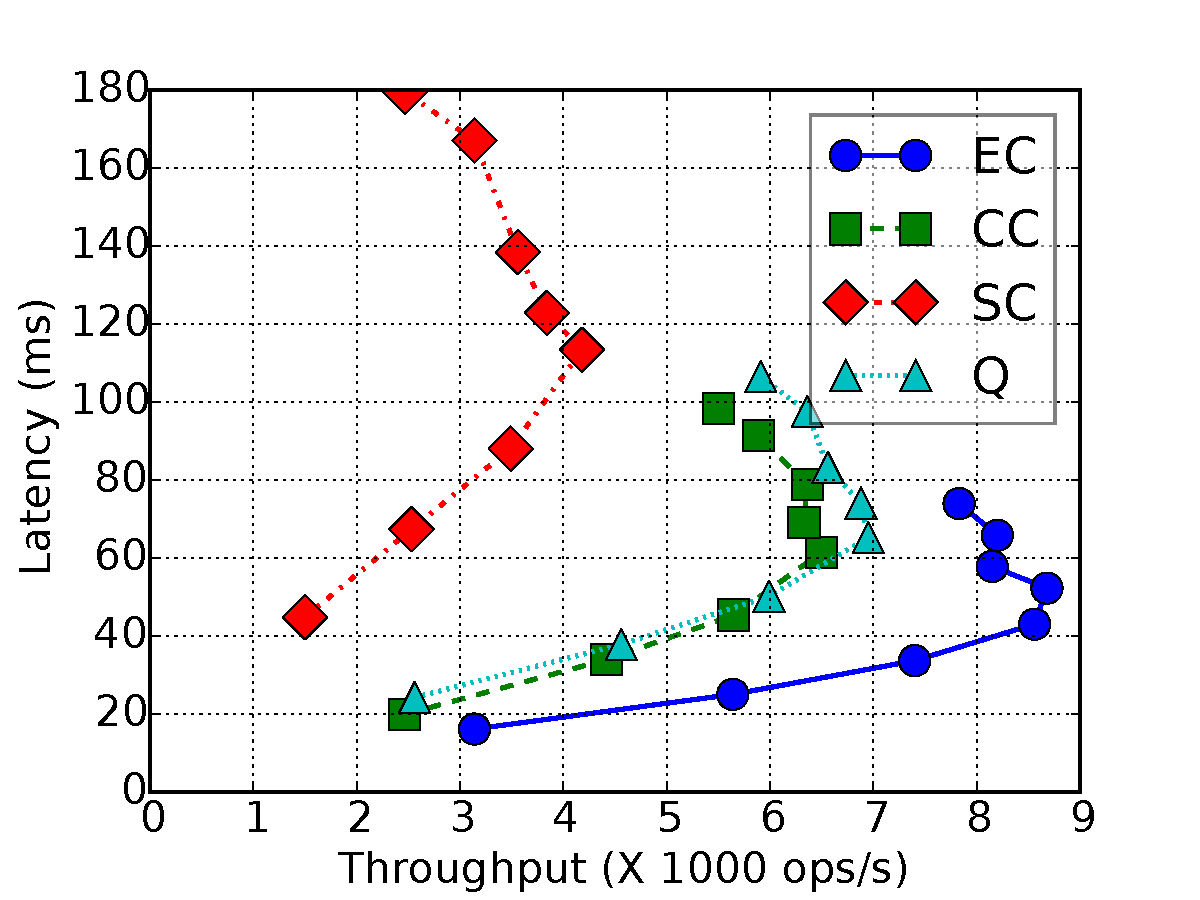
\includegraphics[width=0.24\textwidth]{graphs/BA-tp-vs-lat.pdf}}
  \subfigure[LWW transactions]{\label{grf:LWW-txn}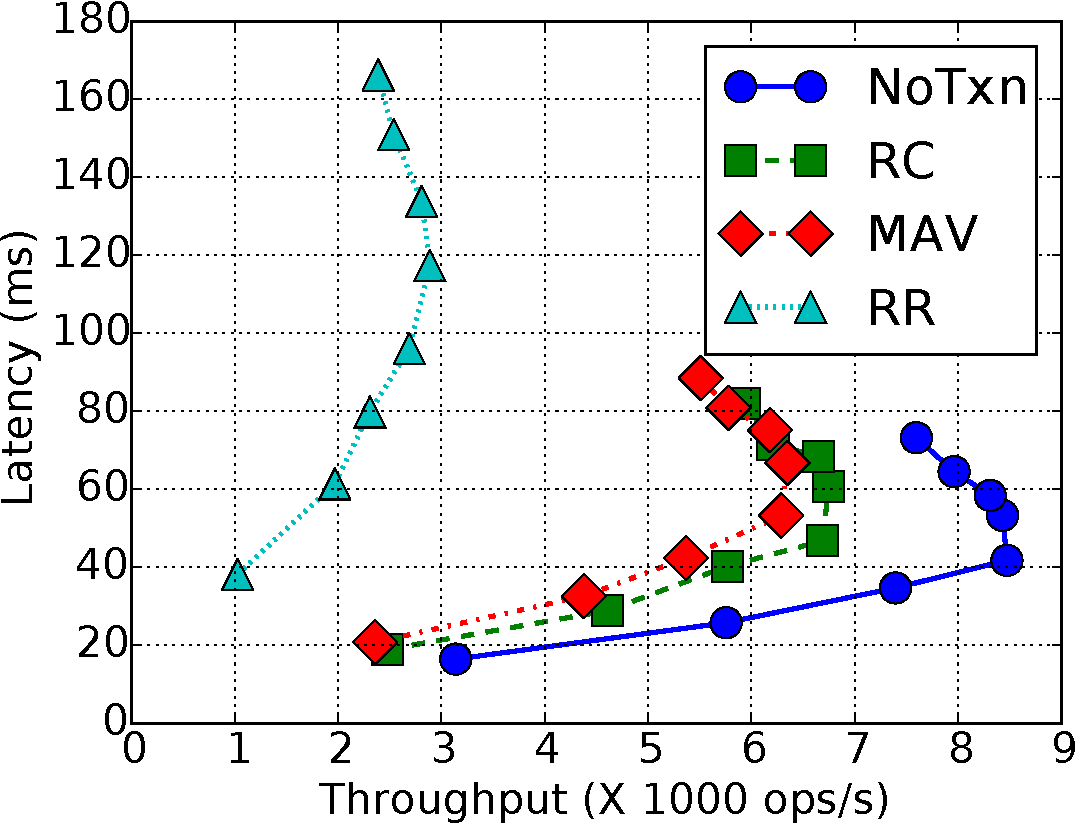
\includegraphics[width=0.24\textwidth]{graphs/LWW-txn.pdf}}
  \subfigure[RUBiS bidding mix]{\label{grf:rubis}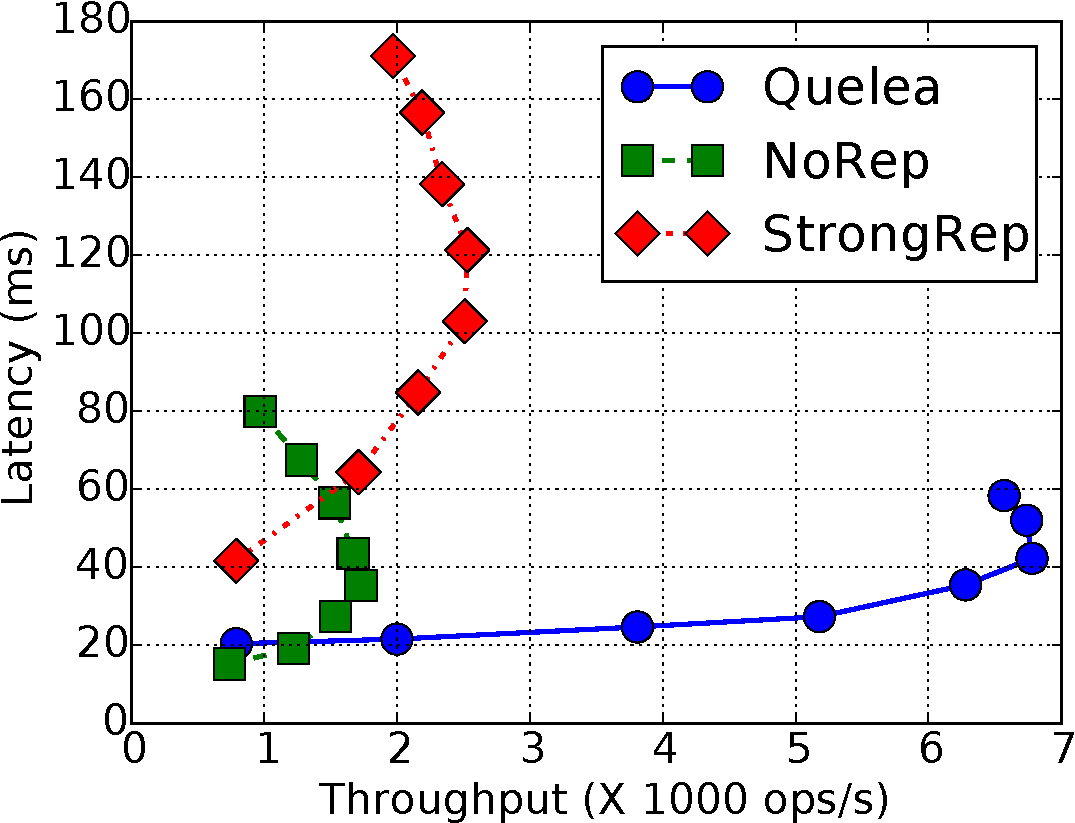
\includegraphics[width=0.24\textwidth]{graphs/Rubis.pdf}}
  \subfigure[Impact of summarization]{\label{grf:summarization}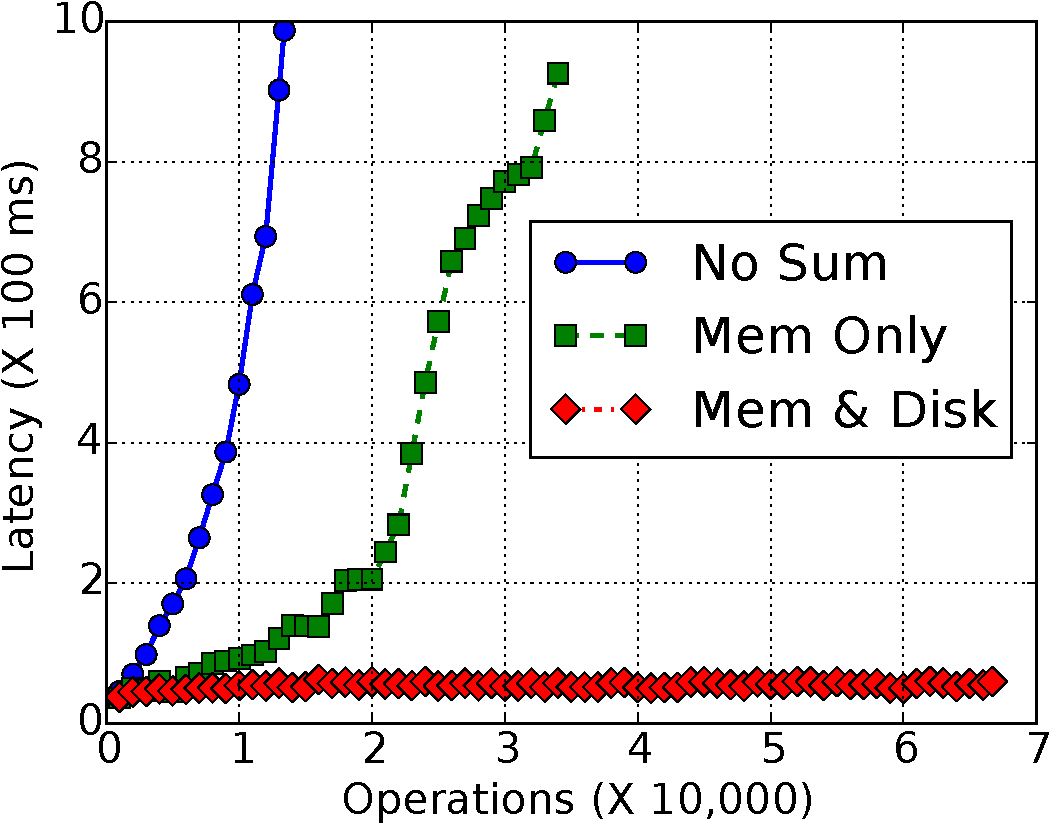
\includegraphics[width=0.235\textwidth]{graphs/summarization.pdf}}
	\caption{Quelea Performance.}
  \label{grf:LWW_perf}
\end{figure*}

Figure~\ref{grf:BA-tp-vs-lat} shows the throughtput vs. latency of operations
in bank account example as we increase the number of clients in \cf{1DC}
configuration. Our client workload was generated using YCSB benchmark~\cite{}.
The benchmark uniformly chose from 100,000 keys, where the operation spread was
25\% withdraw, 25\% deposit and 50\% getBalance, which corresponds to the
default 50:50 read:write mix in YCSB. We increased the number of clients from
128 to 1024, and each experiment ran for 180 seconds.

The lines marked EC and CC correspond to all operations being assigned EC and
CC consistency levels. These levels compromise correctness as withdraw has to
be and SC operation. The line SC corresponds to a configuration where all
operations are strongly consistent; this ensures application correctness. \name
corresponds to our implementation, which classifies operations based on their
contracts. Both \name and SC ensure correctness. However, with 512 clients,
\name implementation was within 41\% of latency and 18\% of throughput of EC,
whereas SC operations had 162\% higher latency and 52\% lower throughput than
EC operations. Observe that there is a point in each case after which the
latency increases while the throughput decreases. This indicates a point after
which the store becomes saturated with client requests.

In \cf{2DC} configuration (not-shown), the average latency of SC operations
with 512 clients increased by 9.4$\times$ due to the cost of geo-distributed
coordination, whereas \name operations were only 2.2$\times$ slower, mainly due
to the increased cost of \cf{withdraw} operations. Importantly, the latency of
\cf{getBalance} and \cf{deposit} remained almost the same. This illustrates the
benefit of fine-grained contract classification in \name.

We compare the performance of different transaction isolation level choices in
Figure~\ref{grf:LWW-txn} using the LWW register. The numbers were obtained
under 1DC configuration. The YCSB workload was modified to issue 10 operations
per transaction, with the default 50:50 read:write mix. Each operation is
assumed to have eventual consistency. \cf{NoTxn} corresponds to a configuration
that does not use transactions. Compared to this RC is only 12\% shower in
terms of latency with 512 clients, where as RR is 2.3X slower. The difference
between RC and \cf{NoTxn} is due to the meta-data overhead of recording
transaction information in the object state. For RR transaction, the cost of
capturing and maintaining the snapshot in an RR transaction is the biggest
source of overhead.

We also compared (not shown) the performance of EC LWW operations directly
against Cassandra (our backing store), which uses last-writer-wins as the only
convergence semantics. While Cassandra provides no stronger-than-eventual
consistency properties, \name was within 30\%(20\%) of latency(throughput) of
Cassandra with 512 clients, illustrating that the programmers only have to pay
a minimal overhead for the expressive and stronger \name programming model.

Figure~\ref{grf:rubis} compares the \name implementation of RUBiS in \cf{1DC}
configuration against a single replica (NoRep) and strongly replicated
(StrongRep) \cf{1DC} deployment. The benchmark was RUBiS bidding mix, which has
15\% read-write interactions, which is representative of the auction workload.
Without replication, NoRep trivially provides strong consistency. However, this
deployment does not scale beyond 1750 operations per second. Strong replication
offers better throughput at the cost of greater latency due to inter-replica
coordination. \name deployment offers the benefit of replication, while only
paying the cost of coordination when necessary.

Finally, we study the impact of summarization in
Figure~\ref{grf:summarization}. We utilize 128 clients and a single \name
replica, with all the clients operating on the \emph{same} LWW register to
stress test the summarization mechanism. We utilize 50:50 read:write mix, and
33:33:33 EC:CC:SC mix. The shim layer cache (mem) of operations is summarized
every 64 updates, while the updates in the backing store (disk) are summarized
every 4096 updates. Each point in the graph represents the average latency of
the previous 1000 operations. Each experiment is run for 60s.

The results show that without summarization, the average latency of operations
increase exponentially to almost 1 second, and only 13K operations were
performed in a minute. Since every operation has to reduce over the set of all
previous operations, with a ever growing set, the operations take increasingly
more time to complete. With summarization only in memory, the performance still
degrades due to the cost of fetching all previous updates from the backing
store into the shim layer. Fetching the latest updates is essential for SC
operations. With both summarizations enabled, we see that the latency does not
increase over time, and we were able to perform 67K operations. This graph
illustrates the importance and effectiveness of summarization in \name.
